% -------------------------------------------------------------------------------- %

\begin{exercise}

Try to reproduce Figure \ref{fig:8.2} on page 165.
Then apply a multi-step algorithm to this problem.
What does the performance comparison look like?

\setcounter{section}{8}
\setcounter{figure}{1}

\begin{figure}[H]
    \centering
    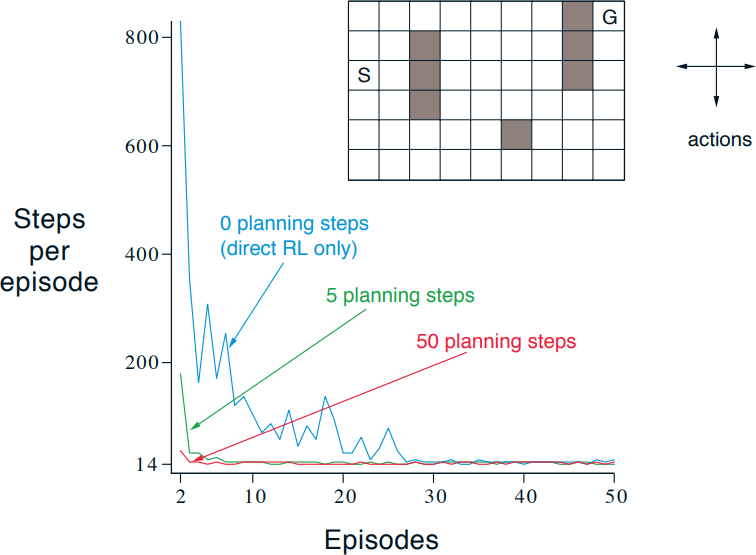
\includegraphics[width = 0.75 \textwidth]{4.44.png}
    \caption
    {
        A simple maze (inset) and the average learning curves for Dyna-Q agents varying in ther number of planning steps ($n$) per real step.
        The task is to travel from $\mathsf S$ to $\mathsf G$ as quickly as possible.
    }
    \label{fig:8.2}
\end{figure}
\end{exercise}

% -------------------------------------------------------------------------------- %

\begin{solution}

\begin{figure}[H]
\centering
\begin{minipage}{.5\textwidth}
  \centering
  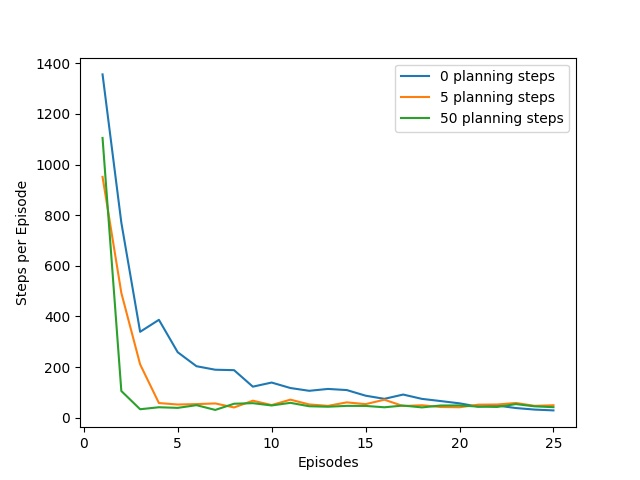
\includegraphics[width=.7\linewidth]{dyna.jpg}
  \captionof{figure}{The recreated graph of the Dyna-Q maze}
  \label{fig:test1}
\end{minipage}%
\begin{minipage}{.5\textwidth}
  \centering
  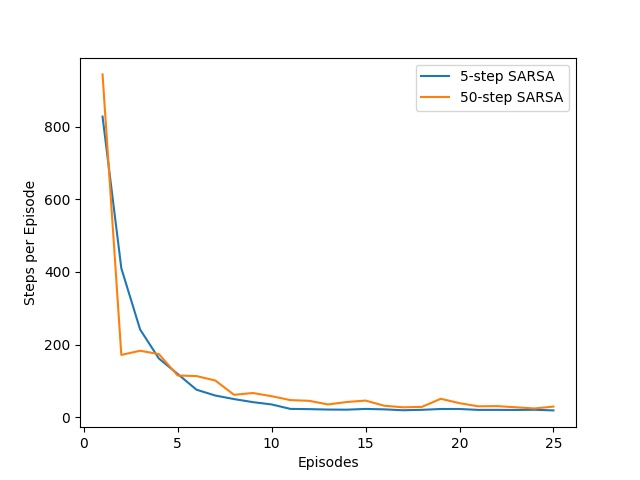
\includegraphics[width=.7\linewidth]{sarsa.jpg}
  \captionof{figure}{n-step SARSA applied to the same maze}
  \label{fig:test2}
\end{minipage}
\end{figure}

The graphs shows a comparison between the methods with values $\alpha = 0.1, \gamma = 0.95$ and $\varepsilon = 0.1$. The number of steps in each episode is the mean over 30 runs.
\end{solution}

% -------------------------------------------------------------------------------- %
